\documentclass[10pt]{article}
\usepackage[T1]{fontenc}
\usepackage{lmodern,amsmath,amssymb,graphicx,hyperref}
\usepackage[margin=.75in]{geometry}
\setlength{\parindent}{0pt}\setlength{\parskip}{6pt}
\begin{document}
\begin{center}{\Large Degree-limited actual whole-chart factors}\\[4pt]
14 November 2026; 29 authored statements\\
Source \texttt{c11739ba2966aa6d269822de35249d83e3254401}
\end{center}
\textbf{Checked construction.} The isolated project builds29 authored statements
without warnings. Pinned shared audit29 declarations/0 extra trusted axioms,
exit0, no generated extras. Import-inclusive fresh replay is running,
not passed. All records unsigned [pcc:unverified].

\textbf{Actual scope.} Use the same completed auxiliary $W$, actual bounded
ports $x,y<2^a$, natural multiplicities, and nonzero signed-grid source node
$t$ with $v_2(t)=i<u\le a$. Matrices explicitly mask noncrossing entries to
zero. The actual fixed negative-pole diagonal is $c$, with $w=v_2(c)$.
No positive multiplicity or nonzero local-first-jet premise is added.

\textbf{Combined grading.} Coefficient $H^b$ of the actual bivariate
geometric approximation has $Z$-grade $b-1$. Dividing by $2^b$ gives
grade $-1$ of the actual constructed right factor $V_{(r,b),y}(Z)$:
\[
 v_2([Z^n]V_{(r,b),y})\ge n-1,
\]
with zero coefficients admitted at every weight. The grade is derived from
actual denominator slopes and the existing actual normalized chart, rather
than supplied as a good-factor hypothesis [pcc:unverified].

Define $V^{\le k}$ by truncating each actual right polynomial below degree
$k+1$. The coefficient bound gives content-$k$ error. The finite matrix
product error is proved using actual left integrality and sums, then scaled
by $c$. The resulting profile is
\[
 \begin{gathered}
 \operatorname{natdeg}V^{\le k}_{(r,b),y}\le k,\qquad
 \operatorname{Content}_0(V^{\le k}_{(r,b),y}),\\
 \operatorname{Content}_{w+b}(\widehat U_{x,(r,b)}),\qquad
 \operatorname{Content}_{w+k}
   (W^{\rm cross}_{xy}-(\widehat U V^{\le k})_{xy}),\\
 \#\{(r,b)\}=2^u k.
 \end{gathered}
\]
Every label remains charged; $k=0$ is included. Scaled-left integrality
retains $w\ge0$. No full-matrix or origin rank claim [pcc:unverified].

\begin{center}
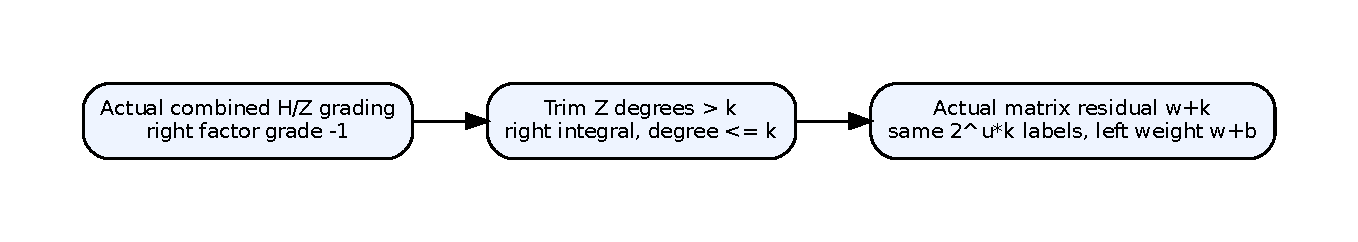
\includegraphics[width=\linewidth,height=1.15in,keepaspectratio]{dependencies.pdf}
\end{center}
\newpage
\begin{center}{\Large Source bindings and complete-cost boundary}\end{center}
\textbf{Exact source map.} The complete Lean statement governs every
hypothesis. Central source-bound records are
\begin{center}\small
\begin{tabular}{p{.63\linewidth}p{.26\linewidth}}
\texttt{actual\_approx\_rows\_mixed}&PCC-20261114-09a254\\
\texttt{actual\_poly\_right\_graded}&PCC-20261114-29f555\\
\texttt{trimmed\_right\_degree}&PCC-20261114-75f9e9\\
\texttt{actual\_degree\_limited\_precision}&PCC-20261114-dbcc3e\\
\texttt{actual\_degree\_limited\_profile}&PCC-20261114-9f4003
\end{tabular}
\end{center}
All29 bindings and source/configuration/gate/trust pins are in
\begin{center}\small
\path{../evidence/claim-pins.json}\\
\path{../evidence/source-freeze.json}.
\end{center}
Gate data is PCC-20261114-fd52a6. Import-inclusive
\texttt{leanchecker --fresh --verbose OrientationDegree} is running;
no completed exit is inferred. All records are unsigned [pcc:unverified].

\textbf{Pinned environment.} Lean4.35.0, CryptoLean and Mathlib revisions:
\begin{center}\small
\texttt{148f5dc389b341401e06d76abe7783c4ccf42f2e}\\
\texttt{cfc55fc58714a59dc06e6e79edc6d1d95140d3c2}.
\end{center}
The source is byte-identical accepted local degree004. Its earlier one-page
report and data36a2d2 remain exact inside Compact106. All four local drafts
and raw builds remain preserved, including a reserved-lambda variable,
omitted definition and ambiguous weightedLeft failures. Accepted004 prints
five central dependencies with only standard foundations, no
\texttt{sorryAx}. No linter or hypothesis was disabled [pcc:unverified].

\textbf{Original mode interface.} Primary D.12--16 uses column tiles
$2^{i+1}$, at most $6M/D_i$ modes per weight, one source/target group for
each mode, and fixed creation-precision representatives. This construction
uses $2^u$ row classes per moment. Its degree bound is not a count of
nonzero modes or a complete entry-computation bound [pcc:unverified].

The separate mode-evidence draft has its own exact local status and is
OUTSIDE these29 statements/audit/replay. Its support/cardinality/negative-
pole width claims do not establish child-network coefficient extraction,
ring transport, immutable creation-precision lifting or the complete
recurrence. The negative-pole fixed-family restriction is not a lower bound
for arbitrary nodes, completions or algorithms.

\textbf{Next accounting.} Charge actual rational coefficient bit sizes,
modular transport into the integral coefficient ring, entry construction at
its creation precision, original mode density, Hermite recovery and every
recursive call. Actual elliptic relation/public finder, field and scalar
extraction, retries and full expected bit cost remain open. No runtime
exponent or sub-exponential algorithm conclusion from degree alone.

\textbf{Sources checked.} KB unavailable as journaled. Read exact
Graded/Mixed/Compact/Node/Higher/Moment proofs and pinned PowerSeries
coefficient/truncation degree APIs, primary D.4.5--6 and original cost/
precision/triage reviews. Standard grading/truncation/matrix algebra reused
without novelty, priority, fastest-method or timing claim.

No native crypto, attack, F4/msolve, timing, scaling, paid or cloud campaign.
The original norm fixture remains unlaunched under its unchanged transport
blocker. No measured data updates canonical IC graphs/leaderboards; the
diagram records proof dependencies. Preserve Compact106/Higher83+final13/
Node90 and all older pins. Protected concurrent PCC histories remain
unresolved; auto-merge stays off. No rechain, signature or prefix waiver.
\end{document}
